\documentclass{article}

% Language setting
% Replace `english' with e.g. `spanish' to change the document language
\usepackage[french]{babel}
\usepackage[fleqn]{amsmath} % Aligner les équations à gauche


% Set page size and margins
% Replace `letterpaper' with`a4paper' for UK/EU standard size
\usepackage[letterpaper,top=2cm,bottom=2cm,left=3cm,right=3cm,marginparwidth=1.75cm]{geometry}

% Useful packages
\usepackage{amsmath}
\usepackage{graphicx}
\usepackage{subcaption}
\usepackage[colorlinks=true, allcolors=blue]{hyperref}

\title{TD8}
\author{IPESUP - PC }
\date{10 Janvier 2024}

\begin{document}
\maketitle



\section{Rappels de cours}
\begin{enumerate}

    \item \textbf{Définitions:}\\[0.1cm]
    \begin {itemize}
    \item Ligne de courant : Courbe de l'espace qui possède en tout point une tangente parallèle à la vitesse du fluide.\\
    \item Tube de courant: Ensemble des lignes de courant qui passent par un contour fermé.\\
    \item Fluide parfait : Fluide sans viscosité.\\
    \end{itemize}
    \item  \textbf{Conservation de la masse : }\\[0.2cm]
$     \frac{\partial \rho}{\partial t} + div(\rho \vec{v}) = 0$ \\

On a souvent $\rho = cste$ , donc $ div(\vec{v}) = 0 $ . \\[0.1cm]


\item \textbf{Accélération particulaire :}
 \\[0.1cm]

$\frac{Df}{Dt} = \frac{\partial f}{\partial t} + \vec{v} \cdot \vec{grad}(f)$\\

$\vec{v} \cdot \vec{grad}(f)$ est un opérateur : \\

$\vec{v} \cdot \vec{grad}(f)$ = $v_x \frac{\partial f}{\partial x} + v_y \frac{\partial f}{\partial y} + v_z \frac{\partial f}{\partial z}$\\

Pour une variable vectorielle, on a : \\[0.2cm]
$\vec{v} \cdot \vec{grad}(\vec{f})$ = $\vec{v} \cdot \vec{grad} (f_x) \vec{e_x} + \vec{v} \cdot \vec{grad} (f_y) \vec{e_y} + \vec{v} \cdot \vec{grad} (f_z) \vec{e_z} $\\

\item \textbf{Equations dynamiques : }\\[0.1cm]

Equation d'Euler: $\rho \frac{D\vec{v}}{Dt} = -grad(P) + \rho \vec{g} $\\[0.1cm] 
\\
On obtient cette équation en appliquant le PFD à une particule de fluide. 

\item \textbf{ Théorème de Bernoulli : }\\[0.1cm]
Pour un Fluide parfait, en Régime stationnaire, dans un écoulement Incompressible , dans un référentiel Galiléen, et si le fluide est hOmogène (FRIGO),  alors on a (sur une ligne de courant): \\[0.1cm]
$P + \frac{1}{2} \rho v^2 + \rho g z = cste$\\[0.1cm]

Si en plus le fluide est irrotationnel, cette formule est vraie partout ! (pas que sur une ligne de courant)
\\[0.1cm]

\item \textbf{Formule utile: }
\end{enumerate}



\\[0.1cm]
$\vec{v} \cdot \vec{grad}(v) = \vec{rot}(\vec{v}) \times \vec{v} + \vec{grad(v^2/2)} $



\section{Bulle de cavitation:}



Au sein d'un fluide incompressible, une bulle de rayon $a$, sphérique et vide, est formée à l'instant t=0. 
Ce phénomène peut par exemple se produire à proximité de l'hélice d'un sous-marin. 
On cherche à déterminer l'évolution du rayon de la bulle en fonction du temps.
On notera $a(t)$ le rayon de la bulle. 
On néglige les effets de la pesanteur et on note $P_0$ la pression du fluide loin de la bulle, ainsi que $\vec{v}(r,t)$ le champ de vitesse. 
\begin{enumerate}
    \item Montrer que $v(r,t)=a(t)^2 \frac{1}{r^2} \frac{da}{dt}$. 
    En déduire que l'écoulement dérive d'un potentiel $\Phi(r,t)$ qu'on déterminera. 
    \item Trouver l'équation vérifiée par $a(t)$. 
    \textit{ Indication: on pourra intégrer l'équation d'Euler entre $a$ et l'infini. }
    \item Estimer un temps caractéristique d'implosion. 
    \item Le Titan est un sous-marin civil perdu en mer le 18 juin 2023.
    D'après les enquêteurs, le sous-marin aurait subi une implosion à une profondeur de 3800m. 
    En justifiant que le temps caractéristique calculé précedemment peut être utilisé pour déterminer un ordre de grandeur de la durée d'implosion du Titan, commenter la phrase suivante: 
    " Les passagers ne se sont pas rendus compte de ce qui leur arrivait ". 
    \\[0.1cm]
    \textbf{Donnée: } Les signaux nerveux se propagent dans le corps humain à une vitesse de l'ordre de 50m/s.
\end{enumerate}


\section{Ondes de gravitation}

On considère un bassin rempli d'un fluide incompressible, de profondeur $H_0$ et de longueur infinie.
Un vibreur génère des ondes sinusïdales à la surface de l'eau. 
On note $h(x,t)$ l'altitude de la surface libre à l'abscisse $x$. 
%ksi en latek: \xi
On note $\xi(x,t)$ la perturbation, de sorte que $h(x,t) = H_0 + \xi(x,t)$.
On suppose que les ondes sont de faible amplitude, c'est à dire que $\xi \ll H_0$.
On notera de plus $\xi(x,t)=\xi_0 sin(\omega t - kx)$
On suppose l'écoulement irrotationnel et on note $\vec{v}(x,z,t)$ le champ de vitesse.
\begin{enumerate}
    \item Montrer que le champ de vitesse dérive d'un potentiel $\Phi(x,z,t)$. 
    On cherchera ce potentiel sous la forme $\Phi(x,z,t)=f(z) cos(\omega t - kx)$.
    \item Donner l'équation dont est solution $\Phi(x,z,t)$ et en déduire que $f$ vérifie l"équation ${\frac{d^{2}f}{d z^{2}}}-k^{2}f=0$.
    \item Montrer que $\frac{\partial\phi}{\partial z}(z=0)=0$. Qu'en déduit-on sur $f$ ? 
    \item Montrer que l'autre condition limite s'écrit $\frac{\partial\phi}{\partial z}(z=H_{0})=\frac{\partial h}{\partial t}$
    \item En déduire l'expression de f en fonction de $\xi_0$. 
    \item En déduire l'expression de $\vec{v}(x,z,t)$.
    \item 
    
    On note $(x^*(t), y^*(t), z^*(t))$ les coordonnées d’une particule de fluide. (Noter que la coordonnée $y^*(t)$ restera invariante).
    Montrer que $x^*(t)$ et $ y^*(t)$  verifient le système d’équations suivant :\\[0.1cm]
    $\frac{d x^{*}}{d t}=\frac{\xi_{0}\omega}{\sinh(k H_{0})}\cosh(k z^{*}(t))\sin(\omega t-k x^{*}(t))$\\
    $\frac{d z^{*}}{d t}=\frac{\xi_{0}\omega}{\sinh(k H_{0})}\sinh(k z^{*}(t))\cos(\omega t-k x^{*}(t))$\\

    \item Ce système d’ ́equations différentielle qui ne depend que du temps n’a pas de solution analytique
    dans le cas général. Néanmoins, on observe que les particules de fluide forment des ellipses dont la taille est très petite devant la longueur d'onde.
   On remplace alors $kx^*$ et $kz^*$ par $kx_m$ et $kz_m$, les valeurs moyennes de $x^*$ et $z^*$ dans l'ellipse. 
   Résoudre alors le système d'équations différentielles.

\end{enumerate}

    \section{Tube tournant:} 
    On considère un tube coudé de section circulaire plongé dans de l'eau et tournant autour de l'axe $Oz$ avec une vitesse angulaire $\omega$.
    On suppose l'écoulement irrotationnel.
    Quelle conditions doit on avoir sur $\omega$ pour que ce système fonctionne comme une pompe ? 

    \begin{figure}[h]
        \centering
        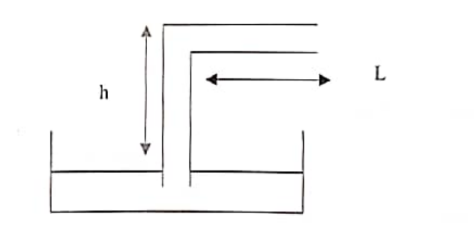
\includegraphics[width=0.4\textwidth]{tube_tournant.png}
        \label{fig:image1}
        \title{Schéma du tube tournant}

      \end{figure}

\section{Vidange d'un réservoir:}

On considère un réservoir de section $S$ et contenant une hauteur d'eau $h$. 
On ouvre une vanne de section $s$ en bas du réservoir et on note $h(t)$ la hauteur d'eau dans le réservoir.
Calculer la durée mise par le réservoir pour se vider. 

\textbf{Bonus: } (Tombé à l'X à l'oral) En combinant cet exercice et l'exercice 2 du TD7, décrire le mouvement d'un camion citerne possédant une ouverture en bas de son réservoir.
        

\end{document}